\documentclass{template/openetcs_report}
% Use the option "nocc" if the document is not licensed under Creative Commons
%\documentclass[nocc]{template/openetcs_article}
\usepackage{rotating,url,color}
%\usepackage[hidelinks]{hyperref}
%hidelinks put some problems on some distributions
\usepackage{hyperref}
\graphicspath{{./template/}{.}{./images/}}
\begin{document}
\frontmatter
\project{openETCS}

%Please do not change anything above this line
%============================
% The document metadata is defined below

%assign a report number here
\reportnum{OETCS/WP7/D7.1~--~00/11}

%define your workpackage here
\wp{Work Package 7, Task 1: ``Primary Toolchain''}

%set a title here
\title{Report on the Final Choice of the Primary Toolchain }

%set a subtitle here
\subtitle{ Decision on the final choice for the means of description (O7.1.4), tools (O7.1.8) and tool platform (O7.1.11)}

%set the date of the report here
\date{September 2013}

%define a list of authors and their affiliation here

\author{Michael Jastram}
\affiliation{Formal Mind}

\author{Marielle Petit-Doche}
\affiliation{Systerel}

\author{all participants of the decision process}
\affiliation{WP7 partners}

% define the coverart
\coverart[width=350pt]{openETCS_EUPL.png}
 
%define the type of report
\reporttype{Deliverable}

\begin{abstract}
This document gives  a description and the results of the first task of WP7. The objectives of the task are to analyze and recommend, means, tools and platform to develop the primary toolchain of Open ETCS.

\end{abstract}

%=============================
%Do not change the next three lines
\maketitle
\tableofcontents
\listoffiguresandtables
\newpage
%=============================


\begin{tabular}{|p{4.4cm}|p{8.7cm}|}
\hline
\multicolumn{2}{|c|}{Document information} \\
\hline
Work Package &  WP7  \\
Deliverable ID or doc. ref. & D.7.1 (including O7.1.4, O7.1.8, O7.1.11) \\
\hline
Document title & Report on the final choices for the primary toolchain \\
Document version & 00.11 \\
Document authors (org.)  & Michael Jastram (Formal Mind), Marielle Petit-Doche (Systerel) and WP7 partners  \\
\hline
\end{tabular}

\begin{tabular}{|p{4.4cm}|p{8.7cm}|}
\hline
\multicolumn{2}{|c|}{Review information} \\
\hline
Last version reviewed & 00.06 \\
\hline
Main reviewers &  \\
\hline
\end{tabular}

\begin{tabular}{|p{2.2cm}|p{4cm}|p{4cm}|p{2cm}|}
\hline
\multicolumn{4}{|c|}{Approbation} \\
\hline
  &  Name & Role & Date   \\
\hline  
Written by  & Michael Jastram & WP7 Task Leader  &  \\
&  Marielle Petit-Doche & WP7-T7.1 Sub-Task Leader  & \\
& Cécile Braunstein & &  \\
& Uwe Steinke & &  \\
& Stanisla Pinte & &  \\
& Alexander Stante & &  \\
\hline
Approved by & Michael Jastram & WP7 leader & \\
\hline
\end{tabular}

\begin{tabular}{|p{2.2cm}|p{2cm}|p{3cm}|p{5cm}|}
\hline
\multicolumn{4}{|c|}{Document evolution} \\
\hline
Version &  Date & Author(s) & Justification  \\
\hline  
00.01 & 08/07/2013 & M. Petit-Doche &  Document creation  \\
00.02 & 18/07/2013 & M.~Jastram, C.~Braunstein & Complements in § 3 \\
 &  & U. Steinke & Draft version of appendix A \\
00.03 & 19/07/2013 & M.Petit-Doche & Complements in § 2 and § 4 \\
00.04 & 31/07/2013 & M.Jastram & Significant work in §§1, 2, 3 and 4 before review. \\
00.05 & 13/08/2013 & M.Petit-Doche & Github issues taken into account: 80, 84, 87, 88, 89, 90(partial), 96 107 \\
00.06 & 15/08/2013 & Stanislas Pinte & significant review of Papyrus-ERTMSFormalSpecs-Eclipse proposal \\
00.07 & 26/08/2013 & U. Steinke, M. Petit-Doche & Cleaning in all the document Github issues taken into account: 82, 83, 90, 100, 112, 116, 119 \\
00.08 & 29/08/2013 &  M. Petit-Doche & Cleaning in all the document Github issues taken into account: 85, 99, 100, 123, 124, 126 \\
00.09 & 03/09/2013 & M. Jastram,  M. Petit-Doche & Cleaning in all the document Github issues taken into account: 62, 102, 126 (partial), 132, 136 \\
00.10 & 03/09/2013 & A. Stante & Description: Image of SysML / Classical B toolchain updated. Minor updates in text. \\
00.11 & 03/09/2013 &  M. Petit-Doche & Cleaning in all the document Github issues taken into account: 86, 108, 116 \\
\hline  
\end{tabular}

% The actual document starts below this line
%=============================


%%%%%%%%%%%%%%%%%%%%%%%%%%%%%%%%%%%%%%%%%%%%%%%%%%%%%%%%%%%%%%
%%%              My macros (=> Sylvain Baro)               %%%
%%%%%%%%%%%%%%%%%%%%%%%%%%%%%%%%%%%%%%%%%%%%%%%%%%%%%%%%%%%%%%
\newcommand{\tbd}{\colorbox{cyan}{\%\%To Be Defined\%\%}}
\newcommand{\tbc}{\colorbox{cyan}{\%\%To Be Confirmed\%\%}}
\newcommand{\todo}[1]{\colorbox{cyan}{\%\%{#1}\%\%}}
\newlength{\origindent}

\newenvironment{issue}{
        \begin{quote}
        \begin{itshape}Open Issue.
}{
        \end{itshape}
        \end{quote}
}

\newenvironment{comment}{
        \begin{quote}
        \begin{itshape}Comment.
}{
        \end{itshape}
        \end{quote}
}

\newenvironment{justif}{
        \begin{quote}
        \begin{itshape}Justification.
}{
        \end{itshape}
        \end{quote}
}


\newenvironment{todo_comment}{
        \begin{quote}
        \begin{itshape}\textcolor{green}{Todo:}
}{
        \end{itshape}
        \end{quote}
}
%%%%%%%%%%%%%%%%%%%%%%%%%%%


% Start here

\mainmatter



%-----------------------
\section{Motivation}
%-----------------------

%-----------------------
\section{Scope of the document}
%-----------------------

%----------------------
 \section{Reference documents}
%----------------------- 
\begingroup
%\renewcommand{\section}[2]{}%
\renewcommand{\chapter}[2]{}% for other classes
  \bibliographystyle{plain}
  \bibliography{wp7_bibliography}
\endgroup
%%% Local Variables: 
%%% mode: latex
%%% TeX-master: WP7-Toolchain_architecture"
%%% End: 


\chapter{Results on means and tools for primary toolchain}
\label{sec:results}

\section{Proposed Toolchains}

This chapter describes the proposed toolchains and the selection process for finding them.

There were three toolchain proposals in total (Figure~\ref{fig:proposals}).  These are:

 \begin{figure}[b!]
  \centering
  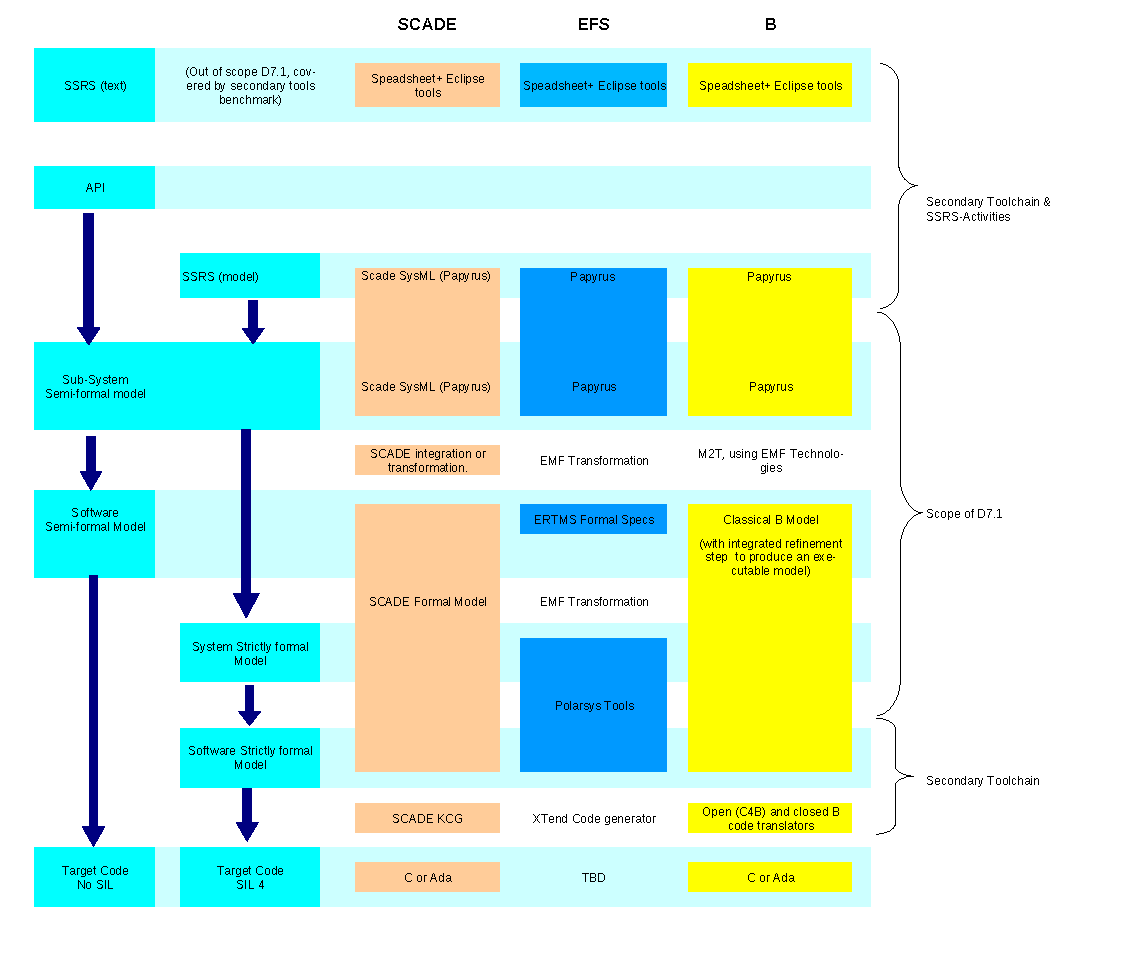
\includegraphics[width=\linewidth]{images/compare-toolchains.pdf}
  \caption{Proposed Toolchains}
  \label{fig:proposals}
\end{figure}

\begin{description}

\item[SCADE.] A SCADE-based primary toolchain would consist of the two tools Papyrus and SCADE.  An integration between the tools already exists, and both tools cover all activities.  The biggest advantage is that there would be little additional work necessary to cover the primary toolchain.  The biggest drawback of this solution is the fact that SCADE is not open source.

\item[ERTMS Formal Specs (EFS).] An EFS-based primary toolchain would mainly consists of the Papyrus, EFS and additional components from the Eclipse ecosystem, looking at Polarsys for guidance.  It is not clear if and how the formal models could be modelled with this toolchain.  The biggest advantage of this approach is that it is open source, and that a significant portion of Subset 26 has already modelled with EFS.  The biggest drawback is that it is not clear how the integration with Papyrus would look like, that EFS is only partly ported to Eclipse, and that it is not clear how laborious the tailoring of the Eclipse-based formal modeling tools would be.

\item[B.] In contrast to the previous proposals, this one starts bottom-up, starting with the assumption that code generation from B models is possible and practical.   This toolchain proposes working with B on the bottom two layers, but leaves open how these are connected to the Papyrus-based top.  The biggest advantage of this approach is that the resulting model will be usable, and that there is a rich existing ecosystem for B, both open source and commercial.  The biggest drawback is that there are many blanks to fill in, which may require significant development work.

\end{description}

\section{Selection Process}

The selection process consisted of the six steps shown here, with more detail being provided below.

\begin{description}

\item[Benchmarking. (Section~\ref{sec:benchmarking})] Project partners were asked to step up and perform a benchmark of the tool of their choice.  The proposals were checked against D2.1 (State of the art) to make sure that no important tools were missed (or if so, why).  Not all benchmarks were completed, CORE, Why3 and UPPAAL dropped out.  Further, after completing the benchmark, GOPPR, GNATprove and Petri Nets decided to run, due to the evaluation results.

\item[Assessment (Section~\ref{sec:assessment}).] Each Benchmark was assessed by its author and by two additional assessors (in the case of Petri Nets and GNATprove, there was just one assessor).  The assessment quantified evaluation criteria, resulting in a report consisting of hundreds of scores for each completed benchmark.

\item[Decision Meeting(Section~\ref{sec:decision_meeting}).] A decision meeting took place to eliminate tools and to start looking at possible tool configuration that would form the primary toolchain.  During this meeting, Enterprise Architect (SysML) was also eliminated, in favor of the open source alternative Papyrus.  Further, Papyrus/SCADE was identified as one promising toolchain.  Further, Papyrus had been selected as the tool for the Sub System Semi-formal model.

\item[Composition of Toolchains (Section~\ref{sec:composition_of_tool_chains}).] With the number of tools reduced significantly and one selected tool (Papyrus), team members were invited to propose concrete toolchains covering the primary toolchain.  This resulted in two more proposals, in addition to Papyrus/SCADE.

\item[Documenting the Decision (Section~\ref{sec:documenting_the_decision}).] This deliverable documents the three toolchains, as well as their respective strength and weaknesses.  As has been determined a long time ago\footnote{Tool Selection Process: https://github.com/openETCS/model-evaluation/wiki/Benchmark--to-evaluate-model-and-tools\#tool-selection-process}, we didn't expect a clear single ``best'' solution.  The document will steer the upcoming activities to prevent redundant or unnecessary work.

\item[Final Choice of Toolchain.] Which of the three competing toolchains will eventually be used for openETCS shall be decided six month after D7.1 the latest (as documented in the tool selection process).  Note that this may not be one of the three suggested, but could also be a composition of elements of the three toolchains.

\end{description}

\subsection{Benchmarking}
\label{sec:benchmarking}

The following thirteen tools have been selected for benchmarking:

\begin{tabular}{ p{0.5\linewidth} p{0.5\linewidth} }
SCADE & ERTMSFormalSpecs \\
SysML with Papyrus & SysML with Enterprise Architect \\
Classical B with Atelier B & Event-B with Rodin \\
System C & Petri Nets$^\ddagger$ \\
GOPRR$^\ddagger$ & GNATprove$^\ddagger$ \\
UPPAAL$^\dagger$ & Why3$^\dagger$ \\
CORE$^\dagger$
\end{tabular}

$\dagger$ The evaluation of three tools was stopped prematurely.  They are mentioned in \cite{WP7_O719}, but are not evaluated.  They dropped out for the following reasons:

\begin{description}
\item[CORE] The tool is not open source and difficult to obtain, it seems possible to cover the same task with an open-source approach as SysML.
\item[Why3] Gnat-Prove covers at least the same service and seems more efficient.
\item[UPPAAL] It is a tool dedicated to the verification and validation of time-constraints properties, for example joined with SystemC. It has been proposed for the benchmark on secondary tools (T7.2).
\end{description}

$\ddagger$ At the end of the evaluation, three others approaches have been discard from the primary toolchain:

\begin{description}
\item[GOPPR] SysML seems a better candidate to offer the same services.
\item[GNATprove] According the results, GNATprove has been proposed to joined the evaluation of secondary tools (task T7.2).
\item[Petri Nets] However it is a well-known formal approaches, more recent approaches seems more adapted to the goals of the project.
\end{description}

\subsection{Assessment}
\label{sec:assessment}

Each Benchmark was assessed by its author and by two additional assessors (in the case of Petri Nets and GNATprove, there was just one assessor).  This has been documented in \citep{WP7_O719}, which contains the ``raw data'', as well as some rudimentary aggregation of the data and some analysis.

The criteria in \citep{WP7_O719} were derived from WP2 requirements and quantified on scale from 0 to 3.  The results were recorded as the sum of the author and the two assessors, resulting in a score from 0 to 9 for each criteria.  The benchmarks with only one assessor have been adjusted by interpolating the score, shown in parentheses.

To give an idea of the results, Table~\ref{tab:phaseresults} shows the aggregated result of the benchmark for process phases.  These results must be taken with a grain of salt: This aggregation simply averages all relevant scores, thereby giving all criteria equal weight.  This is an unrealistic (and dangerous) assumption.  In fact in the case of the criteria ``open source'' it created a real problem.  As Open Proof is the foundation of openETCS, using a closed-source tool with no open alternative should be a show stopper.  But this does not show in the results of \citep{WP7_O719}.

Further, not all criteria could be quantified easily, resulting in surprising and suspicious results.  For instance, the assessments of Papyrus and Enterprise Architect sometimes differed drastically, even in areas, where the notation (and not the tool) was concerned.  This was not expected, as both tools support the same notation.  This means that the results must be inspected carefully, before drawing conclusions.

 \begin{table}
  \centering
\begin{tabular}{|l | c | c | c | c | c | c | c | c | c | c |}
\hline
&  \rotatebox{90}{GOPRR} & \rotatebox{90}{ERTMSFormalSpecs} &  \rotatebox{90}{SysML with Papyrus} &  \rotatebox{90}{SysML with EA} &  \rotatebox{90}{SCADE} &  \rotatebox{90}{Event-B} &  \rotatebox{90}{Classical B} &  \rotatebox{90}{System C} & \rotatebox{90}{Petri Nets} &  \rotatebox{90}{GNATprove} \\
\hline 
System Analysis & \textcolor{blue}{5} & 1     & \textcolor{magenta}{7} & \textcolor{red}{\textbf{9}} & 3     & \textcolor{red}{\textbf{9}} & 3     & 2 & \textcolor{red}{\textbf{6(9)}}  & 2 (3) \\
\hline
Sub-system formal design  & \textcolor{red}{\textbf{9}} & \textcolor{red}{\textbf{9}} & \textcolor{blue}{6} & \textcolor{magenta}{7} & \textcolor{red}{\textbf{9}} & \textcolor{red}{\textbf{9}} & \textcolor{blue}{5} & \textcolor{blue}{5}  & \textcolor{red}{\textbf{6(9)}}   & 3 (4) \\
\hline
Software design  & \textcolor{red}{\textbf{9}} & \textcolor{green}{0} & \textcolor{blue}{6} & \textcolor{magenta}{7} & \textcolor{red}{\textbf{9}} & \textcolor{blue}{6} & \textcolor{red}{\textbf{9}} & \textcolor{red}{\textbf{9}} & \textcolor{red}{\textbf{6(9)}}   & \textcolor{red}{\textbf{6(9)}}  \\
\hline
Software code generation  & \textcolor{red}{\textbf{9}} & \textcolor{green}{0} & 3     & 3     & \textcolor{red}{\textbf{9}} & 3     & \textcolor{red}{\textbf{9}} & \textcolor{blue}{6} & 2 (3) & \textcolor{red}{\textbf{6(9)}}   \\
\hline
\end{tabular}
  \caption{Use of the approaches during process phases}
  \label{tab:phaseresults}
\end{table}

\subsection{Decision Meeting}
\label{sec:decision_meeting}

On July 4th, a WP7 workshop took place with the objective of choosing suitable tools for the toolchain.  To ease the process, the results from \citep{WP7_O719} were condensed into Figure~\ref{fig:results}.  The vertical stripes represent the individual tools.  The length and position of the stripe is determined by Table~\ref{tab:phaseresults}: The bar only covers area with a score of 6 or higher.

 \begin{figure}
  \centering
  \fbox{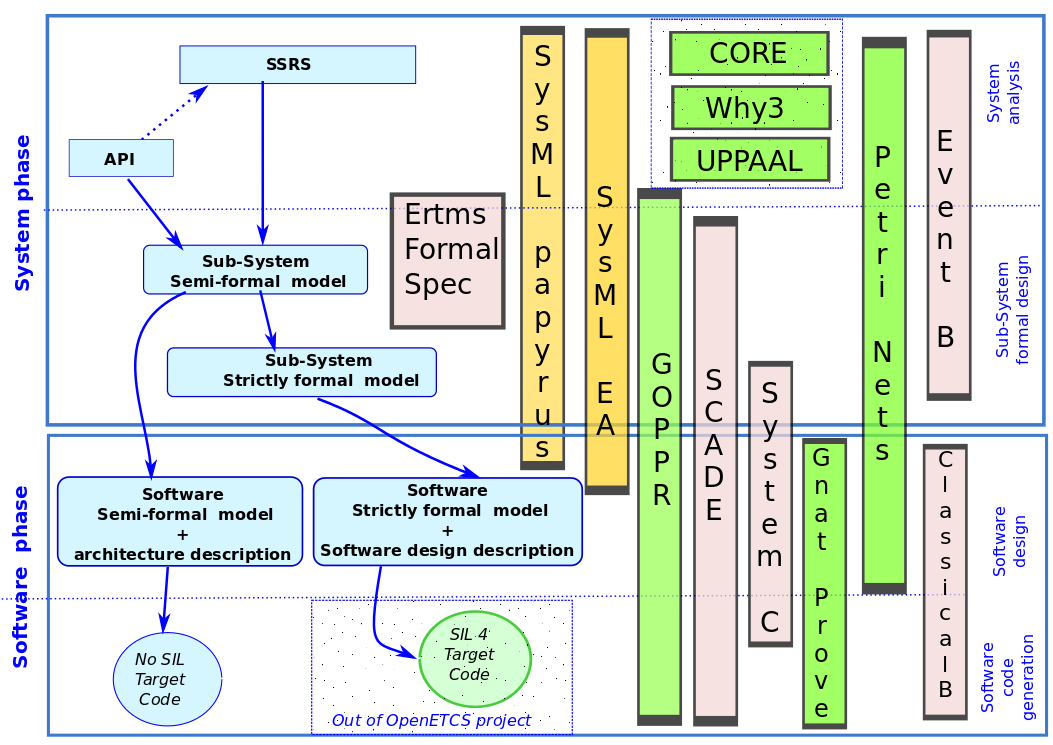
\includegraphics[width=\linewidth]{images/First.png}}
  \caption{Results of candidates}
  \label{fig:results}
\end{figure}

\subsubsection{SysML}

Using the available data as the foundation, the objective was to narrow the choices down as much as possible.  One obvious redundancy was the availability of two SysML tools, Papyrus and Enterprise Architect. After discussion of pros and cons of each, the partners agreed that Papyrus covers better the objectives of the project, especially the open-source requirement. 

Further, by vote, all the partners agree on the use Papyrus/SysML to cover the higher level of the  OpenETCS V-cycle.

\subsubsection{Short List}

Due to the evaluation and discussion during the decision meeting, the partners agreed on a short-list of six approaches. These are shown in red in Figure~\ref{fig:results}. and include the following:

\begin{tabular}{ p{0.5\linewidth} p{0.5\linewidth} }
SCADE & ERTMSFormalSpecs \\
SysML with Papyrus & System C \\
Classical B with Atelier B & Event-B with Rodin
\end{tabular}

\subsection{Composition of Toolchains}
\label{sec:composition_of_tool_chains}

One toolchain was already suggested during the Paris meeting, namely Papyrus and SCADE.  Nevertheless, partners had the chance to propose additional toolchains using the tools from the shortlist.  It was necessary to find alternatives, as one severe weakness of the Papyrus/SCADE solution had already been pointed out in Paris: By not being open source, this solution would miss one of the main objectives of openETCS.

Two more toolchains have been proposed, resulting in three toolchains in total.  These have been documented by their respective owners in the appendix.

\subsection{Documenting the Decision}
\label{sec:documenting_the_decision}

What has been documented so far is a promising foundation for an openETCS primary toolchain.  However, it is not clear on how to proceed from here, as there are multiple competing avenues.  Resources in the project are thin and should be employed wisely.  Therefore, Section~\ref{sec:decision} contains an elaborate analysis with clear decisions that will guide the activities of the next six month, ensuring that we will choose the best option for openETCS while minimizing risk.






\chapter{Results on tool platform}
The tool platform should provide mechanisms to integrate various
tools. The tool platform is not the primary nor secondary tools, nor
the tool chain. It is the support for the tool chain implementation,
it shall help to integrate the tools into a seamless tool chain.
The evaluation will focus on the integration capabilities of the tool platform.
\begin{todo_comment}
Description of the candidates by Cecile Braunstein
\end{todo_comment}

\section{Initial list of candidates}
\begin{itemize}
\item Eclipse 
\item TopCased/Polarsys
\item RTP-Cesar
\item Mono/.NET 
\item SCADE
\end{itemize}

After a first round, Mono/.NET and SCADE were discard because they do
not comply to our tool platform definition.  RTP-CESAR was also
discard, the maturity of this project is not yet usable. Finally,
{\bf Eclipse with the modeling framework (EMF)} has been chosen as a tool
platform, the possibility to use Polarsys and take some part of the
TopCased tool chain as well as which version of Eclipse  and EMF to choose are
discussed in the next sections.  

Eclipse can also integrate framework, It has also be decided that any
framework added to the Eclipse platform within the OpenETCS tool chain
should be documented (version, usage ...) and clearly justify.

\section{Eclipse}
Eclipse is an open source Tool Platform originally developed at
IBM. It has been explicitly designed as an extensible platform to
enable different tools to exchange data and share common
functionality. Additionally Eclipse is a rich open source ecosystem
with a variety of frameworks for different purposes, such as
versioning, code generation, language support and many more. The
Eclipse Modeling Framework (EMF) as a top level project bundles all
modeling frameworks at Eclipse. Additionally it technically provides a
common data format for modeling purposes. Originally it has
implemented the OMG Standard Meta-Object Facility (MOF) and has then
be reduce to the OMG standard essential MOF (eMOF). EMF provides
model-driven approach to develop modeling languages. It allows to
define custom meta-models and generate code form them. Additionally it
provides common features such as command-based editing and XMI
serialization for generated models. In the following we show how
Eclipse and EMF aligns with the openETCS requirements.

\paragraph {Open Source}
All Eclipse core components including EMF are open source and under
the Eclipse Public licenses, which allows for commercial use and is
compatible to the EUPL. The Eclipse Foundation and the Eclipse
Development process assure the management of the intellectual
properties for all Eclipse projects. Additionally all Eclipse projects
follow a common infrastructure and process allowing external partners
to contribute and maintain projects. 

\paragraph{Long-Term Maintenance}
The Eclipse Foundation also provides infrastructure and a process for
Long-Term Maintenance for all Eclipse projects. It enables users of a
technology to contract service providers to maintain current and older
versions of these technologies. These service providers do not
necessarily have to be committers on the original projects.

\paragraph{Portability}
Eclipse itself is implemented in Java and therefore portable to all
major operating systems. The underlying UI technology SWT is
implemented for all major and even most uncommon window kits. As SWT
uses native widgets, the performance of the UI is close to native
applications. The Eclipse Java IDE has a user based of several million
developers, which ensures, that the platform runs stable on the
supported platforms. Since version 4.2, EMF is part of the core
platform. However, EMF does not contain any OS specific components and
is therefore highly portable.

\paragraph{Tools Interoperability}
The Eclipse Platform has been explicitly designed to enable various
tools of the software lifecycle to collaborate. It provides
mechanisms, such as a service oriented architecture and extension
points to enable the communication between different parts of a tool
chain. EMF is well-suited as a common data-format. The collaboration
of a large number of tools is shown and validated in the various
Eclipse packages, which are released in the yearly release train.

\paragraph{Modularity}
Eclipse is based on OSGi, a standard for modularization of Java
applications. The Eclipse OSGi runtime Equinox is the reference
implementation of OSGi. OSGi enables to modularize a system, in this
case the tool chain. Additionally it allows to specify the API of
modules and the dependencies between them. Additionally, the existing
platform provides many possibilities to be extended by new
features. The extensibility and OSGi as an underlying technology allow
fully customizing the Eclipse Platform. Existing pieces and frameworks
can be added to a tool chain, new parts can be developed.

\paragraph{Framework Support}
Over the last ten years, a rich ecosystem of frameworks has developed
around the Eclipse Platform. All these frameworks are developed under
the EPL and checked for IP cleanliness. Eclipse frameworks cover all
different kinds of purposes, however there is a strong focus in
support for tool development and modeling. Modeling technologies are
almost all compatible with EMF as a common data format. Technologies
provided by Eclipse projects include:
\begin{enumerate}
\item Textual Modeling and DSL (e.g. Xtext)
\item Language Support (e.g. CDT, JDT)
\item Source Code Versioning Clients (e.g. Egit, Subclipse, Subversion)
\item Model Repositories and Versioning (e.g. EMFCompare, EMF Diff/merge, EMFStore and CDO)
\item Code Generation (e.g. Xpand, Xtend)
\item Model Transformation (e.g. ATL, QVT)
\item Model Development Tools (e.g. Papyrus, OCL, RMF, Sphinx, eTrice)
\item Graphical Modeling (e.g. Graphiti, GMF)
\item User Interfaces (e.g. JFace, Databinding, EMF Client Platform, EEF)
\item ALM Tooling (e.g. Mylyn)
\end{enumerate}


\section{Version Management}

\section{Topcased and Polarsys}

Topcased is a tool for systems engineering, based on Eclipse and various Eclipse projects.  Polarsys is a project concerned with the long term support of the Topcased tool chain.  There is an overlap between Topcased and the openETCS tool chain.  There is also an overlap between the objectives of openETCS and Polarsys:

\textbf{Topcased and openETCS tool chain.} Both, Topcased and the openETCS tool chain are based on Eclipse.  Further, the openETCS tool chain will definitely use Papyrus, which is also part of Topcased.  And last, both are concerned with covering all aspects of the V-Model, although for different domains (aviation vs. rail).

\textbf{Polarsys and openETCS.}  The objectives of Polarsys and openETCS overlap significantly as well: Both are concerned with tools in a safety-critical domain, requiring tool qualification, etc.  They are also concerned with long term support through open source.

\subsection{State of Topcased and Polarsys}

While the state of the art document mentions Topcased \cite{}, it was not evaluated as a whole.  Merely the Papyurus component of Topcased was evaluated, but a newer version than the one used by Topcased.

Topcased is using a fork of an old version of Papyrus (Ver. 0.8.2) which is no more supported by the CEA (actual version 0.10.X) and, as the CEA is not part of Topcased, no more code development over this version/Topcased will be done by CEA.  Unfortunately, the development on Topcased modeler (forked version of Papyrus) is not so active anymore: 60 commits on the 3 last months (as of July 2013) against more than 1600 commit for Papyrus.  Further, the actual version of Papyrus have been greatly improved with respect to stability since version 0.8.2, and some stability issues may have not been corrected in Topcased.

To conclude, Topcased requires Eclipse 3.7.2 Indigo (1.5 year-old version) which is no more supported by the Eclipse foundation.  Some part of Topcased initiative (plugins/add-ons) may still be very useful to the openETCS project, so we will reach out to the Polarsys community to see whether there is an interest in aligning versions for long term support.  The versions currently used in Topcased are not suitable for the openETCS tool chain, unfortunately.




% (mj) a macro for clearly marking decisions as such.
\newcounter{decision}
\newcommand{\decision}[1]{
\begin{center}
\begin{tabular}{ p{13cm} }
\stepcounter{decision}\textbf{Decision~\arabic{decision}}  \\
\hline
\multicolumn{1}{|p{13cm}|}{#1} \\
\hline
\end{tabular}
\end{center}
}


\chapter{Decisions}
\label{sec:decision}

As anticipated there is not one single tool choice done by WP7 partners. This has the advantage of reducing risk (if a tool does not work out), but the disadvantage of potentially wasting resources and being unfocused.  The objective of this chapter is to summarize results of analyses ( in section \ref{sec:swot}) and the decisions and to propose a work plan that leverages the advantage of having multiple tools, while reducing the risks resulting from this. (see section \ref{sec:dec}.  However, the choice of the tool platform was easy and unanimous.

\section{SWOT Analysis}
\label{sec:swot}

By looking a the strengths, weaknesses, opportunities and threats (SWOT) of each toolchain, we will get a qualitative impression on what we could gain with each solution, and what the risks are.

\subsection{SCADE SWOT Analysis}

\subsubsection{Strengths (SCADE)}

The biggest strength of SCADE by far is that it works ``out of the box'', barely any tailoring is required.  SCADE has been developed for systems engineering, and this is exactly the right field of application.  Further, a Papyrus integration is already available, so little work has to be done here.  Another strength is the fact that some of the secondary tool activities are covered by SCADE as well.

\subsubsection{Weaknesses (SCADE)}

The biggest weakness of SCADE is a show stopper: SCADE is not open source, and as no open source alternative exists, openETCS would miss its open proofs objective.

\subsubsection{Opportunities (SCADE)}

Using SCADE would doubtless increase the chances of success of the modeling activities.  Thus, SCADE is an excellent backup plan.  By nominating SCADE as a backup, we would ensure damage control: A successful model, even if not created with open tools is preferable to no model at all.

There is another opportunity: by dangling the chance to adapt SCADE and potentially opening a large market segment, Esterel (manufacturer of SCADE) may decide to open SCADE --- at least enough for our purposes.

\subsubsection{Threats (SCADE)}

There is the real threat that Esterel is encouraging us to adapt SCADE under the premise of opening parts of SCADE to be compliant with open proofs.  If such discussions would breakdown, after modeling has already started, we'd have a problem.

\subsection{ERTMS Formal Specs SWOT Analysis}

\subsubsection{Strengths (EFS)}

EFS is open source.  Even better, a significant portion of the ETCS specification has already been modeled using the tool.  The creator of the tool (ERTMS Formal Specs) is available in the project and has project resources for WP7, which should result in fast turnaround during development.

It has already been proven that all features of the ETCS specification can be modeled.

EFS has been developed as a commercial tool and is based on real-world needs in the rail industry.

\subsubsection{Weaknesses (EFS)}

EFS has originally been written using the .NET platform.  Even though a prototype based on Eclipse EMF exists, a significant amount of work is required to make it truly user friendly.  However, it should be possible to work during a transition phase with the old tool.

As the notation of EFS is more of a domain-specific language (DSL), a debate has been going on whether EFS is ``formal enough''.  This is not a big problem, as the model could be extended with fully-formal models in relevant places.  A bigger question is how the integration of the various models would be realized.  There won't be a clear answer on that, until we try it out.

Last, the ``lower part'' of the toolchain is citing technologies that need a significant investment of energy before they can be used.  For instance, Xtend is a programming language, which is not doing anything domain-specific.

\subsubsection{Opportunities (EFS)}

The main opportunity is to safe time and resources, as a significant portion of the ETCS specification has already been modeled.  Another is the certainty that a commercial partner will be engaged in the ongoing activities, even after the end of openETCS.

\subsubsection{Threats (EFS)}

The continuation of the toolchain, as shown in Figure~\ref{fig:ERTMSSolutionsAlt_1}, leaves a lot of questions open.  Compare that to the much more concise description of the B-approach in Figure~\ref{fig:classical-b-toolchain}.  Due to the ambiguity there is a significant risk that the model integration won't work as shown.

\subsection{B SWOT Analysis}

\subsubsection{Strengths (B)}

B is proven in the rail industry, where it has been deployed successfully.  There is also a strong body of academic research that can be taken advantage of.

There is a decent amount of tooling already available, both open source and commercial.  However, an almost complete open toolchain has been suggested in Table~\ref{tab:classical-b-tools}, with the Atelier B type checker being the only exception (see Weaknesses below).

There is B-related expertise in the consortium, ensuring that questions can be answered and that there is a commercial incentive.

\subsubsection{Weaknesses (B)}

Atelier B is not Eclipse-based, and Appendix~\ref{sec:sysML-B} points out this shortcoming.  On the positive side, it is available on all relevant platforms (Windows, Mac, Linux).

There is also the Atelier B type checker, which is not open source.  Finding an open replacement for this relatively small component would be one mandatory activity.

While B is well-suited for modeling state-based systems, it is not clear how continuous modeling (e.g. breaking curves) would be realized.


\subsubsection{Opportunities (B)}

B could be the sweet spot between using a commercially proven approach (like SCADE), while still residing in the open source realm (like TOPCASED).  And as there are more options available, both open and closed, the risk is lower.

\subsubsection{Threats (B)}

Acceptance may be the biggest problem, as B is a ``hard core'' formal notation, which is considered hard to read.  We must be prepared to train the users and ensure that they accept it beforehand.

\section{Decisions}
\label{sec:dec}

In the following, we will document a number of decisions that follow from our analysis and that will guide the activities until the end of 2013.

The tools covered here must allow working with the four models shown in Figure~\ref{fig:main_process}.


\subsection{Decision on the tool platform}
\label{sec:decision_platform}

\decision{By vote in Paris on July 4th, 2013, all the partners agree on the use of \textbf{Eclipse} as tool platform. }

 Which version of Eclipse will be used is up to the implementing team (WP7.3).  The last release is Kepler 4.3, launched the 26 of June 2013.


\subsection{Papyrus/SysML}

\decision{By vote in Paris on July 4th, 2013, all the partners agree on the use Papyrus/SysML to cover the highest level of the OpenETCS V-cycle.}

All proposed toolchains will use SysML with Papyrus.  To keep things as flexible as possible, it would be desirable to use SysML in exactly the same way for all approaches.  The B team suggested to create modeling guidelines, and to build a validator for validating the SysML model accordingly.

\decision{All three teams will work together to create modeling guidelines that will apply to all three toolchains.  If this turns out not to be possible, they should create a superset guideline, with extensions for the three approaches.}

\subsection{SCADE}

The analysis shows that we have two promising open proposals (EFS, B), and a third non-open proposal, that is extremely powerful (SCADE).  Considering the constraints of the project, it is clear that SCADE should only be employed if everything else fails.  It is a ``Plan B'' that we should be grateful for, as it may allow us to make openETCS at least a partial success, in case of a larger tool crisis (of whatever nature).  Therefore, we decide:

\decision{The SCADE toolchain will be the ``Plan B'' toolchain, to be employed if ``all else fails''.}

\decision{Therefore, activities on the SCADE toolchain will be suspended for the time being.}

If we are in a real crisis (this will hopefully never happen), we'll have to put relatively little effort into migrating whatever has been done to the SCADE toolchain.  This will be particularly true if we carefully define the scope of the Papyrus component.


\subsection{Aligning EFS and B toolchains}

For better or worse, there is no clear winner between the EFS and B toolchains.  We will know more when the rubber hits the road --- when we start modeling.  Therefore, modeling activities should start as soon as possible with a well-defined case study.

\decision{As the toolchains are being built, modeling will start immediately on a small, well-defined case study, which will represent a subset of the spec.  The model will cover the tool from top to bottom, thereby demonstrating that the toolchain actually works as advertised.}

It is conceivable to continue with the radio subsystem that has been used for the benchmarking, but the modeling expert may suggest a better case study.

It is quite conceivable that no clear winner emerges, but that individual components show unexpected strengths or weaknesses.  Therefore, the toolchain must first define clear interfaces, similar to what the B team already hinted at in Figures~\ref{fig:classical-b-toolchain} and \ref{fig:classical-b-transformation-alternatives}.  Again, there is no reason not to look for similarities between the two open toolchains and to align the interfaces, wherever it makes sense.  For instance, if the Polarsys tools are not performing as expected, they may be replaceable by B tools.  Therefore:

\decision{All toolchains shall clarify their architecture, keep it as modular as possible and align interfaces between them, wherever it makes sense.}

\subsection{Intermediate solution and migration path}

\begin{comment}
Issue \#79 openned by Uwe Steinke to discuss here :


WP 7 is in the obligation to provide and supply all other WPs with an intermediate tool chain until the preferred tool chain becomes operabel. The reason is to enable the other WPs to work productivly.
Additionally, there must be a migration path between the intermediate tool chain and the preferred one, that assures that the results produced with the intermediate tools can be transferred automatically.

The intermediate path has to be specified in this document.

\end{comment}

\section{Conclusion}

While there was some discontent in the team of not having one single solution to move forward with, we simply have to turn this to our advantage.  Having options helps us reduce risk, and by aligning the activities, we prevent our effort from dissipating.  We believe that the documented decisions will act as high-level guidelines for achieving this goal.

The previous section \ref{sec:dec} gives the actual decisions taken by WP7 and project partners.
However, decisions or points of view have been given by the leaders of other workpackages and are summed up in the sequel.

\subsection{WP3 point of view}

\paragraph{WP3 leader point of view (issue \#109):}
\emph{Indeed, ALSTOM, as modeling WP leader, needs now to organize WP3 kick-off meeting and ressources working within a clear framework and objective. With D7.1 conclusion as it is now, WP3 ressources are working now in the tools they want to work on without clear strategy nore objective.
Therefore, ALSTOM proposed following D7.1 conclusions to be :
1 - Despite the fact it is not fully open tools, "SYSML / SCADE" is the baseline primary tools chain to be used for any modeling activity within the frame of the OpenETCS project unless other agreement and.or decision not late than January 2014
2 - In order to allow availability of another complete full OpenETCS Tools chain, complementary analysis and work will be carried out on the 2 other options "SYSML/EFS/Eclpse Polarys" and SYSML / Classical B" for final decision on "OpenETCS" Tools chain not late than January 2014
Such conclusion is likely to avoid dispersion of WP3 ressources that lead to impossibility to manage modeling WP while keeping intact the possibility for the other candidate tools chain to be adopted if confirmed as complete and usable as the only today's available fitted for purpose "SYSML / SCADE" solution.}


\subsection{WP4 point of view}

Some decisions have been made by the WP4 partners regarding VnV and safety activities. these decision have been announced during the decision in Paris on July 4th, 2013:

\decision{WP4 is going to consider the artifacts of "SysML+ Scade" toolchain for the first round of verification and validation launched in July 2013.}

\decision{For the following rounds, starting in February 2014, WP4 will adapt the verification and validation activities to the models and code provides by WP3.}




%%%%%%%%%%%%%%%%%%%%%%%%%%%

\appendix

\chapter{SysML and SCADE}
\label{sec:sysML-Scade}

\section{Description of the approach}

Diagram \ref{fig:SysML_SCADE_Toolchain} illustrates the most important components and operational relationships of a system and software modeling toolchain based on SysML, Papyrus, SCADE and Eclipse. 
All components and links shown with solid lines are available, while the dashed ones are intended to be implemented within the openETCS project. 


\begin{figure}[htbp]
	\centering
		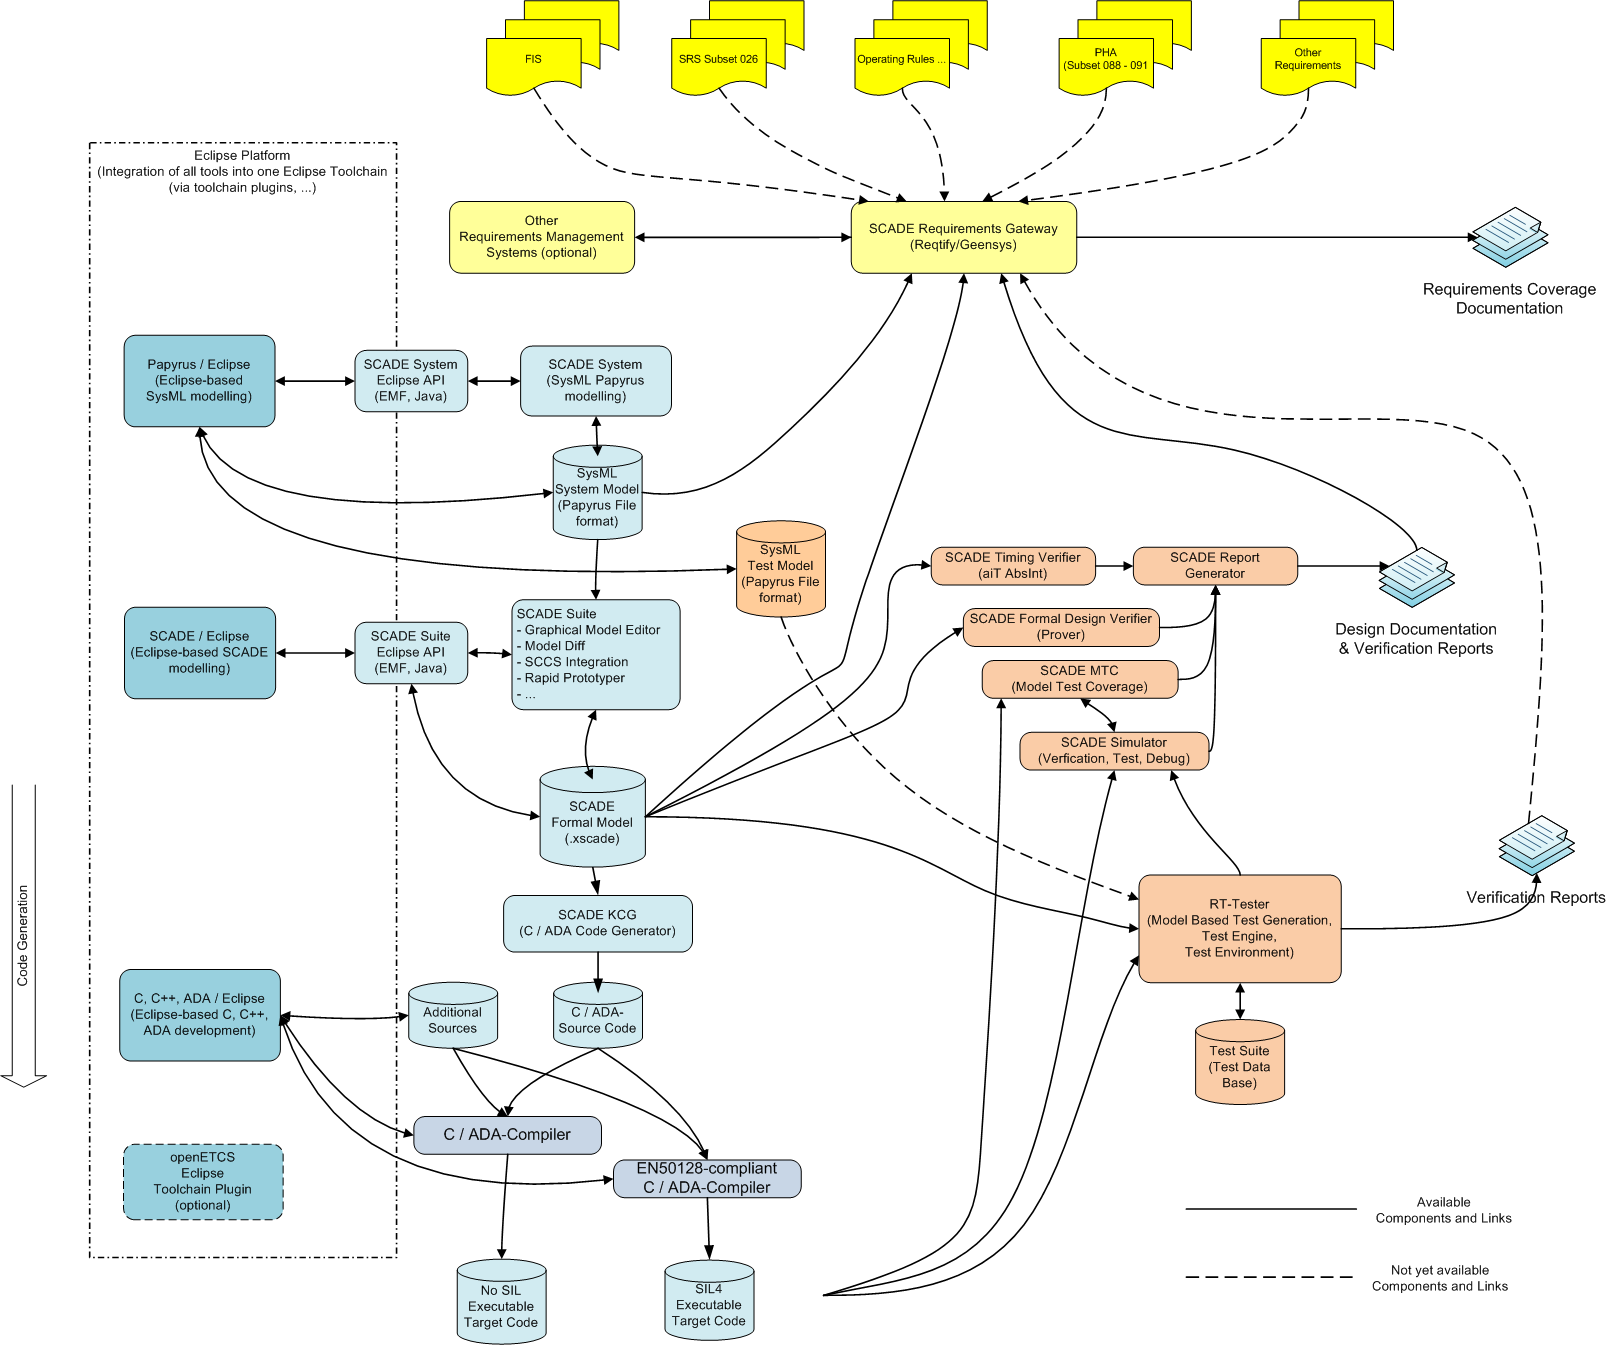
\includegraphics[width=1.10\textwidth]{images/SysML_SCADE_Toolchain.png}
	\caption{SysML SCADE Toolchain}
	\label{fig:SysML_SCADE_Toolchain}
\end{figure}


The diagram colors are chosen related to the colors in figure \ref{fig:main_process}: 

\begin{itemize}
	\item Requirements and requirements management components in yellow
	\item "Blue" openETCS design process ( see figure \ref{fig:main_process}) elements in light and dark blue
	\item Eclipse is painted dark blue
	\item Verification elements in red
\end{itemize}

Within the following paragraphs and subsections a short description of this approach will be given by walking through the tool chain and the design process. 

\subsection{Requirements management}
\label{sec:RequirementsManagement}

The SCADE Requirements Management Gateway is based on Reqtify from Geensoft / Dassault Systems and serves to collect and link all requirements from the openETCS input documents and related objects as design and verification documents, model and source code artifacts, test cases, test protocols etc. It supports impact analyses and generates requirements traceability and requirements coverage reports. 
If needed for the openETCS process, it can be complemented with other requirement management systems and already comes with interfaces to these. ProR for example could be integrated in this way. 


\subsection{Semi-formal System and Subsystem Modeling with SCADE System / Papyrus}
\label{sec:SemiformalModelling}

SCADE System is an integration of Papyrus into the SCADE IDE intended for SysML system modeling. It allows to modelize the interactions and hierarchical dependencies between the various parts of a complex system through design elements representing functions, data and interfaces. 
 
The idea is to model system structures, data types / data dictionaries, inputs, outputs, interfaces and relationships between blocks with SysML and transfer it to native SCADE for behavioral modeling automatically. Since Papyrus and SCADE System are using the same file formats, there is no prevention of using all SysML capabilities that Papyrus supports, but in this case without automatic transfer to native SCADE. 

SCADE System supports SysML Block Definition Diagrams (BDD) and	Internal Block Diagrams (IBD).

More details about the relationship between Papyrus and SCADE System: 

\begin{enumerate}
	\item SCADE System incorporates Papyrus, but SCADE System is more than Papyrus, as outlined in the following list. 
	\item SCADE System enhances Papyrus with functionalities on top: 
	
	\begin{itemize}
		\item Report Generator: Generation of design documents out of the SysML model
		\item Model Check: user expandable checker on SysML models (OCL rule checking, …)
		\item Model Diff: Semantic comparison of models
		\item Interface to requirements management (Reqtify)
		\item Synchronization with SCADE Suite
	\end{itemize}
	
	\item The idea of SCADE System is to ease the work for system and software architects.  SCADE Systems users don’t need so deep knowledge and experience of UML, SysML and …profiles as native Papyrus requires, so that architects or rail engineers, that are not UML experts, are able to work with. Therefore, SCADE System tailors Papyrus in several aspects:
	
	\begin{itemize}
		\item Cleaned up views and user interface and less chances of doing things wrong compared with native Papyrus.
		\item Support for designing blocks (BDD, IBD), relationships and data flows/interfaces between them (as Papyrus).
		\item Support for data types, data dictionaries (as Papyrus).
		\item Allocation of functions (as Papyrus).
	\end{itemize}
	
	\item Actually, SCADE System does not support behavior modeling, but has it on the road map for the next year.
	\item SCADE System uses the same file formats as Papyrus, so that SCADE System and Papyrus files are exchangeable in both directions. SCADE System simply hides SysML artifacts it does not support. This gives the opportunity for:
	
	\begin{itemize}
		\item Using SCADE System for non-UML/SysML experts (architects and rail engineers)
		\item Using Papyrus for UML/SysML experts software experts
	\end{itemize}
	
	\item For integration with Eclipse, SCADE System (as well as SCADE Suite) comes with an Eclipse EMF API including the enhancements on top of Papyrus
\end{enumerate}

With the exception of the synchronization with SCADE Suite, the mentioned easements and enhancements may also be achievable with Papyrus by tailoring and added functionality.
For openETCS, behavioral modeling seems to be necessary for a rather complete model on SysML level. 
Therefore, SCADE System, because ready to use right now, could be chosen for architectural modeling and SSRS matters at the beginning and then continued with Papyrus, when a tailored Papyrus variant becomes available.  

\subsection{Formal Modeling with SCADE Suite}
\label{sec:FormalModellingwithSCADESuite}

SCADE Suite integrates all modeling, verification and supporting SCADE tools under the roof of the SCADE IDE. The components relevant for descending part of the development "`V"' process are

\begin{itemize}
	\item SCADE Suite Editor (Graphical and textual modeling)
	\item SCADE Requirements Gateway Integration (Linking of model artifacts with requirements)
	\item SCADE Model Check (model syntax check)
	\item SCADE Model Diff (model comparison)
	\item SCADE Simulator (graphical debugging, simulation and testing) 
	\item SCADE Rapid Prototyper (quick control and display elements for rapid prototyping, optional)
	\item SCADE Code Generator KCG (C / ADA code generation)
	\item SCADE Reporter ( (Design) report generator)
\end{itemize}

The most important tools for modeling are editor and code generator. The others mentioned are mainly verification tools, but very useful and practically indispensable for agile development.

At least, to cover all elements of the "blue" design process in figure \ref{fig:main_process} a C / C++ / ADA compiler is required. 
For building not safety-relevant executables any C-Compiler (gnu c, ...) is suitable, for safety relevant executables the compiler must be compliant with EN50128.   

\subsection{Model Verification}
\label{sec:SysML_SCADE_ModelVerification}

The verification of openETCS SCADE models can be performed with the "`red"' components shown in diagram \ref{fig:SysML_SCADE_Toolchain}. Most of them are part of SCADE System or SCADE Suite:

\begin{itemize}
	\item SCADE Simulator: The SCADE Simulator should be used in an agile iterative development process for a steady accompanying verification of the modeling work. Simulator test scripts allow executing verification suites for the models automatically. Via its automation and co-simulation interface it is able to be integrated in the openETCS tool chain. 
	\item  SCADE Model Test Coverage MTC: The MTC serves to determine structural model test coverage while executing test scenarios. Instead of measuring code coverage on the generated code, it works on the model structure directly. The MTC tool is automatable. 
	\item SCADE Design Verifier: The verifier performs formal proving and bases upon a model checker from from Prover Technology AB.  
	\item SCADE Timing Verifier: Execution timing verification based on aiT from AbsInt.
	\item SCADE Report Generator: Generation of design reports for SCADE Suite and SCADE System model as well as for verification results. 
	\item RT-Tester: Test engine and environment with model based test case generation and interface to SCADE, see openETCS contributions of the University of Bremen. The ability to derive test cases from a test model complements the verification tool chain with model based testing capabilities.  
\end{itemize}
  

\section{Description of the approach for OpenETCS design process}

The approach as specified in the previous subsections (Chapt. A0) (insert ref xxx ) covers all elements of the "blue" design process ( see figure \ref{fig:main_process}) 
by using the SCADE tool chain including requirements management, semi-formal system and formal subsystem/software modeling, code and executable generation. 
An Eclipse integration is provided (see following Chapt. xxx ). 

\section{Integration of the approach with SysML/Papyrus}

Because SCADE System bases on Papyrus mounted into the SCADE IDE and uses native Papyrus file formats, a seamless integration with SysML / Papyrus is available.
Models can be edited with both, Papyrus and SCADE System and therefore exchanged in both directions. 

Behavioral modeling has to be done with Papyrus until supported by SCADE System as announced for the near future. 

A thrilling question for the openETCS process might be, if and - if yes - which of the artifacts on system level should be modeled with SysML, that can not be transferred to native SCADE automatically. 


\section{Integration of the approach with Eclipse}

All SCADE tools can be run and controlled via command line and/or via automation interfaces. 

SCADE System (SysML modeling) and SCADE Suite (SCADE modeling) already come with Eclipse API plugins based on EMF. These enable to access (read and modify) the model project information, meta and model data from within Eclipse. 
The plugins additionally display the model structure, but they don't show the model graphics in Eclipse. 

If graphical modeling should be done within Eclipse, this has to be implemented by openETCS. It is in doubt, if the effort for this activity would be applicable; without any effort, the SCADE editor should be used instead. 
 
Nevertheless, the provided Eclipse integration is worthwhile to supply all openETCS users, that are not directly working on the SCADE models, with an integrated Eclipse tool chain. 
The idea of such an integration is to have one build tool chain, that starts and runs an openETCS executable build process with one button click beginning from all (heterogeneous) sources and performing all necessary model transformations, code and executable generation. 
This could be achieved with an "`openETCS Eclipse Tool Chain Plugin"', implemented as part of the openETCS project with the goals ease-of-use and convenience. 

In summary, an Eclipse integration is available. An optional "`openETCS Eclipse Tool Chain Plugin"' could improve the convenience for openETCS tool chain users. 


\section{Benefits versus OpenETCS requirements}

The most important benefits of the SysML/SCADE approach are: 

\begin{itemize}
	\item seamless integration,
	\item completeness,
	\item maturity,
	\item qualification for safety critical development,
	\item productivity
	\item availability just now.
\end{itemize}
 
The SysML/SCADE approach covers almost all aspects of the openETCS process and lets expect to fill gaps with manageable effort.

Therefore, the modeling work for openETCS can begin immediately. 

Additionally, the SCADE language covers the capabilities of the ERTMSFormalSpec language, so that ERTMSFormalSpecs models could be transferred to SCADE automatically. Nevertheless, this would require a model transformator, that does not exist actually.   


\section{Shortcomings versus OpenETCS requirements}

The SysML/SCADE approach has one drawback: the tools are mainly not open source. 
These facts may help to better come to terms with it:

\begin{itemize}
	\item The SCADE language is documented and very regular. 
	\item The file formats are documented and easy to understand. 
\end{itemize}

Therefore, the SysML/SCADE approach is open for bidirectional transformations to other modeling languages. 


\section{On going work for openETCS project}

The availability of the nearly complete SysML/SCADE tool chain gives the freedom to focus on the few items to clarify: 

The availability of the nearly complete SysML/SCADE tool chain gives the freedom to focus on few items to clarify: 

\begin{itemize}
	\item Since the tool chain offers several capabilities and options, it has to be determined how these shall be used within the openETCS process. 
	\item A justifiable balance has to be found between semi-formal modeling in SysML and formal modeling in SCADE. 
	\item Some aspects of the RT-Tester integration into the tool chain has to be clarified in detail. 
	\item A requirements management has not been set up for openETCS up to now. If ProR is chosen, it has to be interfaced with the shown Requirements Management Gateway with little effort. 
	\item An "`openETCS Eclipse Tool Chain Plugin"' should be implemented (for convenience only).  
\end{itemize}


\section{Conclusion and other comments}

The most challenging question is, how deep the openETCS functionality should be modeled semi-formal and when to start with formal modeling. 
The question could be answered best if focusing on adequacy: A justifiable balance of technical and non-technical aspects as feasibility, complexity, efficiency,  overall effort,  project schedule etc..

Using SysML/Papyrus with SCADE offers two different alternatives for semi-formal modeling:


\begin{enumerate}
	\item Use SysML/Papyrus for semi-formal modeling by utilizing only the SysML language artifacts, for which an automatic transformation to SCADE exists today. The remaining – formal – modeling then has to be done with SCADE. 
Advantage: The interfacing between SysML/Papyrus is done, the tool chain already complete and ready for modeling right now.
Disadvantage: The semi-formal SysML model will not be as comprehensive as the second alternative 2; there will be system aspects that only reside within the SCADE model, but not in the SysML model.
	\item Use SysML/Papyrus for modeling all system aspects as far as justifiable with respect to understandability, maintainability, adequacy and effort. It requires the determination of a suitable subset of SysML to avoid the model becoming unrulable. 
Advantage: This approach leads to a most complete model on SysML level. It allows to benefit from future transformations between SysML and appropriate formal modeling languages, as soon as they may become available. 
Disadvantage: The openETCS project has to implement the transformation tools from SysML to formal modeling languages; for SCADE, that applies to all SysML artifacts not supported by the existing transformators.
\end{enumerate}

In summary, alternative 1 is easy and ready to use and needs little effort. Alternative 2 offers more flexibility on SysML level but needs more effort and time. 
At least, finding a suitable balance between technical and non-technical aspects could answer the question.  

The fact, that the SysML/Papyrus approach already exists and is operable, offers the chance to start the openETCS modeling process just now without delay. 
In parallel, a truly complete open source and open proof openETCS tool chain can be set up without causing unacceptable impact on the modeling work until it becomes mature enough for practical usage. 



\chapter{SysML, ERTMSFormalSpecs and Eclipse/Polarsys}
\label{sec:sysML-EFS}

The proposed approach combines three tools existing today to provide an integrated toolchain, from system design 
to code generation.

\begin{figure}[b!]
	\centering
		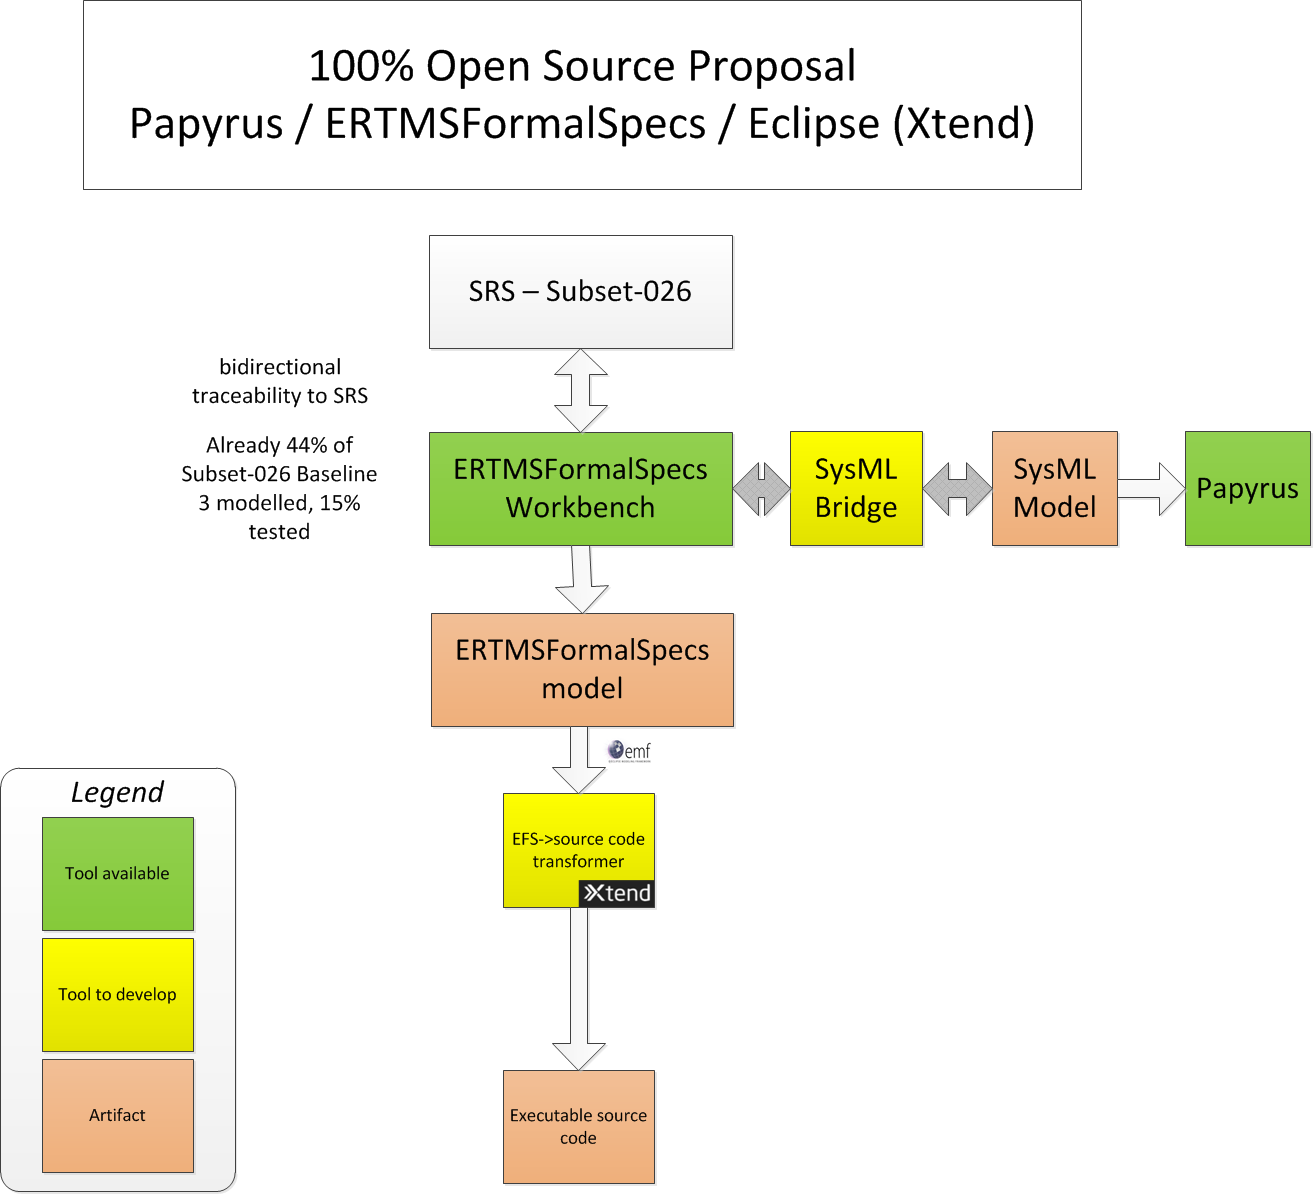
\includegraphics[width=\textwidth]{images/ERTMSFormalSpecsProposal_V3.png}
		\caption{SysML, ErtmsFormalSpec and Eclipse/Polarsys Proposal}
	\label{fig:ERTMSFormalSpecsProposal}
\end{figure}

\section{Description of the approach for OpenETCS design process}

The proposed toolchain is illustrated in Figure \ref{fig:ERTMSFormalSpecsProposal}.

The blue boxes of the overall design process are covered in the following manner:

SRS box: Using Papyrus for visualizing and editing the high-level ERTMSFormalSpecs model design in SysML language. 

Sub-system semi-formal model box: Using ERTMSFormalSpecs to model the complete SRS into a semi-formal model.

Software semi-formal model + architecture description box: Shall be done inside the ERTMSFormalSpecs->source transformer box, using XText Eclipse framework.
The ERTMSFormalSpecs->source transformer shall transform the ERTMSFormalSpecs model into target source code. The architecture and software model of generated source code is part of the ERTMSFormalSpecs->source transformer. The actual target language shall be chosen in agreement with WP5 (demonstrator).

Target source code box: This box is covered by the source code generated by the ERTMSFormalSpecs->source transformer. This source code can then be compiled and executed on the demonstrator hardware.

Note: The ERTMSFormalSpecs->source transformer is not available today, and shall have to be implemented in the scope of the OpenETCS project. This is detailed in further Shortcomings and Ongoing work sections.

Note: the ERTMSFormalSpecs->source transformer doesn't neet to be qualified according to CENELEC standards, to fullfill the two following objectives of the OpenETCS project, i.e. 1/ a complete Subset-026 semi-formal model and 2/ generated, non-vital source code running on demonstrator platform (See Section 3. OPENETCS PROJECT – SCOPE OF WORK AND OBJECTIVES in \citep{WP3_WP4_WP7_SafetyMeetingMinutes_April2013})

Note: How SysML is integrated with lower-level layers is an open discussion, applicable to all toolchains (SCADE, ERTMSFormalSpecs, B). Currently, none of them has proposed a complete, workable approach, enabling round-trip engineering between the higher-level design (in SysML) and lower-level (like SCADE model or ERTMSFormalSpecs model). In the meanwhile, without a clear and usable round-trip strategy is defined by the SysML experts (in collaboration with SCADE, ERTMSFormalSpecs, B experts for instance), the bidirectional arrows linking the ERTMSFormalSpecs model and the SysML model are put in grey, are they are subject to further study.

\section{Integration of the approach with SysML/Papyrus}

The proposed approach uses SysML/Papyrus as a visualization tool on the ERTMSFormalSpecs model. A SysML exporter component (yet to be developed) shall transform selected part of the ERTMSFormalSpecs model into SysML artifacts (state machines, interaction diagrams, module diagrams, data flows, etc) in order to improve readability of the ERTMSFormalSpecs model thanks to SysML. 

In a second phase, if changes are brought to the SysML model, the SysML exporter component could be extended in order to provide round-trip engineering between the ERTMSFormalSpecs model and the generated SysML model, so that changes brought to the SysML model are propagated to the ERTMSFormalSpecs model.

Some questions are open:

- What is the optimal mapping between ERTMSFormalSpecs model elements and SysML diagrams and elements, in order to maximize model readability and verifiability? 
- How can round-trip engineering be implemented, to propagate changes brought to the SysML model back to the original ERTMSFormalSpecs model?

\section{Integration of the approach with Eclipse}

SysML/Papyrus is completely based on Eclipse.

ERTMSFormalSpecs supports today an EMF interface, enabling Eclipse-based tools to reuse the existing ERTMSFormalSpecs model.

Technically, ERTMSFormalSpecs is implemented mostly in C\# and .Net (the ERTMSFormalSpecs workbench) and also has a java-based component, capable of exporting the ERTMSFormalSpecs xml model into an EMF store, so that the ERTMSFormalSpecs model can be accessed from the Eclipse world. 

Eclipse/Polarsys tools are also based on Eclipse, raising no integration concerns.

\section{Benefits versus OpenETCS requirements}

The benefits of the SysML/Papyrus/ERTMSFormalSpecs/Eclipse proposal are the following:

\begin{itemize}
	\item As of today, already 44\% of Subset-026 requirements modelled. This proposal enables the OpenETCS project to start with a headstart, instead of nothing.
	\item ERTMSFormalSpecs is a semi-formal candidate to have built-in braking curves modellings and visualization, verified with the ERA model
	\item ERTMSFormalSpecs has very strong support for traceability to the Subset-026, and to the Subset-076 for test cases. More specifically, inside the ERTMSFormalSpecs workbench, every requirements of Subset-026 can be linked to one or more model artifacts. These links are used by the ERTMSFormalSpecs workbench to generate specification coverage reports. Tests from Subset-076 can also be linked to requirements of Subset-026. For more details, see the online ERTMSFormalSpecs User Guide.  Note: traceability to/from SysML and to generated code remains to be addressed (see section ongoing work for OpenETCS project).
	\item ERTMSFormalSpecs has its domain-specific language, which is highly productive to model Subset-026, thanks to its expressivity, illustrated by the primitives
developed for braking curves and scalable, as is demonstrated by the large fraction of the Subset-026 which has been modelled so far
	\item Fully open-source (ERTMSFormalSpecs under EUPL license, others open source). 
	\item ERTMSFormalSpecs model can be transformed automatically to SCADE model (confirmed by ESTEREL Technologies in Munich meeting), allowing to choose SCADE as a code generation backend in case Eclipse/Polarsys would not meet the project requirements
	\item The three elements of the toolchain (Papyrus, ERTMSFormalSpecs and Eclipse) boast an active community of users and are supported by open-source business cases
\end{itemize}

\section{Shortcommings versus OpenETCS requirements}

The shortcomings of the SysML/Papyrus/ERTMSFormalSpecs/Eclipse proposal are the following:

\begin{itemize}
	\item ERTMSFormalSpecs has a perfectible look and feel and lacks graphical rendering of the architecture. \emph{This shortcoming might be addressed with the integration of SysML as a visualization language.}
	\item As of today, the code generation in Eclipse, transforming the ERTMSFormalSpecs in generated source code, is not yet available, and must be developed during task 3.8 of the project. This should be a relatively easy task, as the code generator doesn't need to be qualified according to CENELEC standards (See Section 3. OPENETCS PROJECT – SCOPE OF WORK AND OBJECTIVES in \citep{WP3_WP4_WP7_SafetyMeetingMinutes_April2013}).
\end{itemize}

\section{On going work for openETCS project}

The following elements should be further developed during the OpenETCS project, to alleviate the shortcomings listed above:

\begin{enumerate}
  \item Develop conceptual and technical strategies to integrate SysML with ERTMSFormalSpecs model, going beyond the state-of-the-art. The state-of-the-art in integrating SysML models and industrial (semi-)formal languages being SCADE System, in which only the module, interfaces and dataflows are connected to the lower-level model.
	\item Further develop ERTMSFormalSpecs model to cover 100\% of Subset-026, 100\% of Subset-076, and to fully test the model within ERTMSFormalSpecs. 
	\item Either implement a full eclipse-based version of the ERTMSFormalSpecs workbench for model development, traceability and testing, or improve the ERTMSFormalSpecs user interface to be fully productive for T3.5 and T3.6 tasks
	\item Develop code-generation strategies during T3.8 tasks
\end{enumerate}

Among theses tasks, Task 2 and 4 fit inside the WP3 existing tasks, and do not need additional skills than the ones present in the OpenETCS consortium as of today. Task 1 is also seriously represented in the consortium, in which a lot of SysML experience is present. 

Task 3 (porting the ERTMSFormalSpecs workbench to Eclipse) is a task that falls in the scope of WP7, and for which Eclipse development and integration skills are required.

\section{Conclusion and other comments}

As a conclusion, the SysML/Papyrus/ERTMSFormalSpecs/Eclipse proposal has as 3 key strengths 1/ to be fully available today for the WP3 modelling tasks, which are the most urgent 2/ to already model 44\% of Subset-026, and 3/ to be fully open-source. 

Moreover, it proposes a realistic technical foundation to achieve the WP3 and projects top-priority objectives with the skills and resources available in the project.


\chapter{SysML and ClassicalB}
\label{sec:sysML-B}

This section describes the approach of combining SysML modeling with
the B Method. The technical realization is shown in Figure
\ref{fig:classical-b-toolchain}. Modeling starts in SysML based on the
tool Papyrus. At the current stage of the project, it is undefined
which SysML elements and diagrams will be used. This must be well
defined to ensure that a transformation from SysML to Classical B is
semantically correct. To ensure this, the approach suggest the use of
the \emph{Object Constraint Language (OCL)} or the \emph{Eclipse
  Validation Framework} for validating the SysML model according to
defined modeling guidelines. Such guidelines may restrict the usage of
certain modeling elements and may enforce certain naming conventions.

The validated SysML model will be transformed to a Classical B model
with a model to text transformation language (e.g. Xtend2). That B
model is considered as read-only and is only allowed to be further
refined. From that point, the existing Atelier B toolchain will be
used for refining the model until reaching the implementation
model. Provers support the V\&V activities and the open source code
generator c4g is capable of generating C code.

The proposed toolchain is intended to be a first version. The yellow
boxes in Figure \ref{fig:classical-b-toolchain} indicate non existing
software artifacts that have to be developed within the openETCS
project. Furthermore, it is desirable to move parts from the Atelier B
tool into Eclipse. 

\begin{figure}
  \centering
  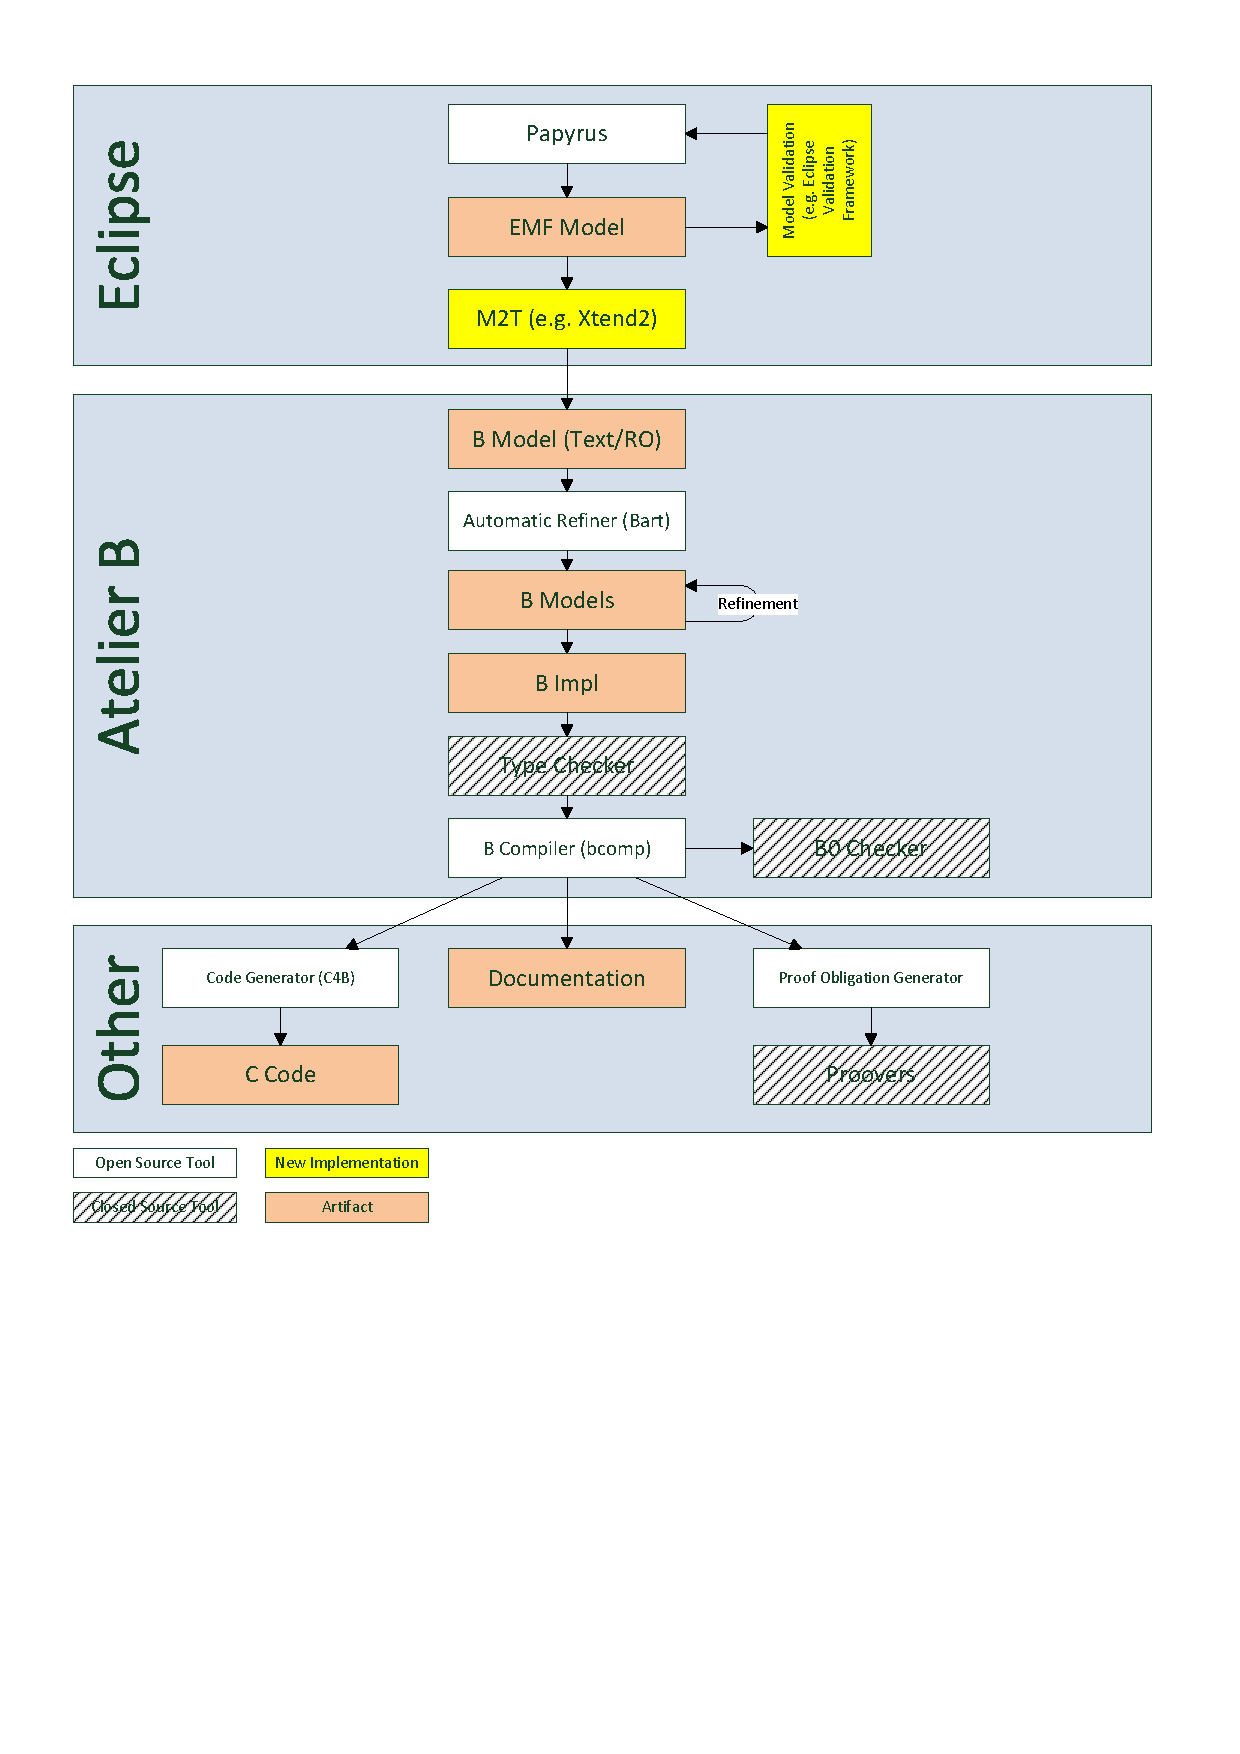
\includegraphics[width=6in]{images/classical_b_toolchain.pdf}
  \caption{Technical overview of the Papyrus and Classical-B toolchain}
  \label{fig:classical-b-toolchain}
\end{figure}


In Table \ref{tab:classical-b-tools} the list of tools used in the
proposed toolchain is given.

\begin{center}
\begin{table}
  \begin{tabular}{ l | l | l }
    Tool                               & License & Link \\ 
    \hline \hline
    Bart (B Automatic Refinement Tool) & GPL & \url{http://sf.net/projects/bartrefiner/} \\ \hline
    Atelier B GUI                      & GPL & \url{http://sf.net/projects/atelierbgui/} \\ \hline
    Bcomp (B Compiler)                 & GPL & \url{http://sf.net/projects/bcomp/} \\ \hline
    C4b (C Code Generator)             & GPL & \url{http://sf.net/projects/c4b/} \\ \hline
    \hline
  \end{tabular}
  \caption{Tools used in the Classical B toolchain}
  \label{tab:classical-b-tools}
\end{table}
\end{center}

\section{Description of the approach for OpenETCS design process}

Taking into account the results presented in Section
\ref{sec:results}, the proposed toolchain completely covers both, the
system phase as well as the software phase (see
Fig. \ref{fig:results}). On system analysis level, SysML with Papyrus
would be used for modeling the SSRS. Also for the sub-system semi
formal model, which will be created during the sub-system formal
design phase, it is proposed to use SysML with Papyrus. The finished
models will then be transformed to B models, to perform further
development steps according to the B method.

For both, the sub-system strictly formal model and the software
semi-formal model it is proposed to use the B method. The development
of the B models will be done by further refining the read-only B
model, generated from the SysML model. It has to be investigated where
\emph{exactly} the transition between SysML and the B model will be
done. In particular, it is currently unclear which SysML language
constructs and diagrams will be used and transformed to B. The
structure described in SysML with \emph{Block Definition Diagrams
  (BDD)} and \emph{Internal Block Diagram (IBD)} are obviously prime
candidates for a transformation to B, but which behavior diagram can
and will can be transformed is still under investigation.

The last part of the development process, the code generation, is
performed with an existing code generator tool.

\section{Integration of the approach with SysML/Papyrus}

On the technical side, the integration will be performed by utilizing
the EMF framework of Eclipse. With an appropriate transformation
language (e.g. Xtend), the SysML model can be transformed to a textual
B model. If it is advantageous to perform the transformation with an
intermediate B meta-model and an a mode-to-model transformation (see
Fig. \ref{}) is under investigation.

The semantic integration of SysML and B method imposes a greater
challenge. There already exist literature regarding the alignment of
SysML and the B method. The work in \cite{} provides such an alignment
focusing on V\&V, which could be used as a base for further research,
which considers in particular the openETCS requirements.


\section{Integration of the approach with Eclipse}

The integration of the proposed toolchain is mainly done as described
in the previous section. After using SysML, the used tool is changed
to Atelier B. This obviously does not correspond to a fully Eclipse
based toolchain. However, this proposal only reflects an initial
toolchain, which could be improved during the project and beyond. The
parts of the toolchain which are user visible and in the first version
realized by Atelier B, could be progressively moved to an Eclipse
based solution. To what extend components from existing solutions
(e.g. the Rodin platform) can be used and if there are enough
resources in the project available, has to be investigated.

\section{Benefits versus OpenETCS requirements}

Both, SysML and the B Methods are accepted in the industry and have
been successful used in the development of safety critical embedded
systems. The B Method was used in Projects like KVB by Alstom, SAET
METEOR or in the driverless metro line 1 in Paris by Siemens
Transportaion Systems (see \ref{} for an extensive list).

Most parts of the toolchain are already available and distributed
under an open source license. The transformation from SysML to B is
the only missing software artifact, that has to be developed for the
first version of the toolchain (see
Fig. \ref{fig:classical-b-toolchain}).

The project consortium includes partner with great expertise in both
languages, SysML and B. By incorporating these expertise, there is a
good chance that the proclaimed goals of openETCS will be achieved.

The modular architecture allows the exchange of certain tools with
more powerful alternatives, even if they are closed-source. For
example, there is a closed source code generator which allows the
creation of ADA or C++ code. This code generator could be used as a
drop-in replacement for the open-source c4b if necessary.

Furthermore, with Eclipse and Atelier-B versions for Windows, Mac OS
and Linux, the most common operating systems are supported by the
proposed toolchain.

\section{Shortcommings versus OpenETCS requirements}

Although the majority of tools used in the toolchain are open-source,
there is a small amount of tools which are closed source (see
Fig. \ref{fig:classical-b-toolchain}). During the project these parts
will be further investigated with the goal to be replaced by
open-source equivalents.



\begin{todo_comment}
Discuss the shortcommings in regards of OpenETCS requirements and expected results.
\end{todo_comment}

\section{On going work for openETCS project}

One of the most important parts is to define a subset of SysML which
can be transformed to Classical B and preserves it semantics. Probably
the other toolchains also need a restricted usage of SysML, therefore
a collaboration on this topic would be advantageous. Furthermore, it
would be ideal if one subset could be defined, which is applicable to
all proposed toolchains.

Another ongoing work is the precise definition of the border between
SysML and Classical B. This work is also linked to the work described
in the previous paragraph, as the border my have implication on
diagrams used in SysML.

The transformation from SysML to Classical B must be planned and
developed within this project. On the implementation part a desirable
skill is the knowledge of transformation languages in Eclipse.

Experience has shown that for model transformations the source model
should be checked according to guidelines. An obvious one is naming as
the source model may allow character combinations that are prohibited
in the destination model.

To show the capabilities and to identify any currently unforeseen
barriers, an early prototype should be developed which illustrates all
steps using an example use-case.

\section{Conclusion and other comments}


%%%%%%%%%%%%%%%%%%%%%%%%%%%

%% Bibliography
% \bibliographystyle{unsrturl}
\bibliographystyle{plain}
\bibliography{wp7_bibliography}


%%%%%%%%%%%%%%%%%%%%%%%%%%%


\end{document}
